\chapter[METODOLOGI PENELITIAN]{\\ METODOLOGI PENELITIAN}
\section{Bahan}
Dalam proses penelitian, diperlukan data yang akan digunakan sebagai bahan pengujian untuk mengukur dan mengevaluasi kinerja metode yang diterapkan. Bahan uji yang digunakan merupakan data dummy yang dirancang dengan struktur menyerupai dataset asli yang diperoleh dari perangkat sensor IoT. Meskipun bukan data asli, dataset ini tetap mempertahankan variabel dan pola data yang umumnya ditemukan pada sensor IoT. Dengan menggunakan dataset dummy, penelitian ini dapat mensimulasikan kondisi real dari hasil sensor tanpa harus bergantung pada data aktual, sehingga memungkinkan pengujian yang lebih fleksibel dan berulang. Selain itu, pendekatan ini juga membantu dalam memahami bagaimana sistem bekerja dalam berbagai skenario yang mungkin terjadi pada sistem berbasis IoT, termasuk skenario yang sulit diperoleh dari data sensor asli. Pembuatan data IoT ini merujuk pada jurnal-jurnal yang membahas mengenai penggunaan sensor baik sebagai single-sensor maupun multiple-sensor. Penulis merancang data tersebut dalam format API yang mengacu pada penelitian yang dilakukan oleh Arief [15] serta Kasera dan Acharjee [33]. 

\begin{enumerate}[label={\alph*.}]
	\item Dummy Single Sensor BME380 \\
	Berdasarkan data yang diperoleh dari jurnal berjudul “Sistem Pemantauan Lingkungan Menggunakan Sensor BME280 Berbasis Internet of Things” [15] oleh Arief, struktur data dalam format JSON yang digunakan adalah sebagai berikut : 
	\pagebreak
	
	\begin{longtable}{|p{.35\linewidth}|p{.60\linewidth}|}
		\caption{Struktur JSON dari Sensor}
		\label{tab:json_sensor} \\  
		\hline
		\multicolumn{2}{|l|}{\textbf{Struktur JSON:}} \\ \hline
		\multicolumn{2}{|c|}{%
			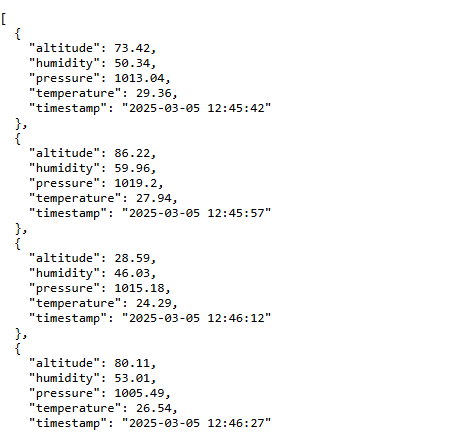
\includegraphics[width=0.8\linewidth, margin=5pt 10pt 5pt 10pt ]{gambar/Metodologi/StrukturJson.png}
		} \\ \hline
		\textbf{Parameter} & \textbf{Keterangan} \\ \hline
		\texttt{altitude} & Posisi vertikal (ketinggian) suatu objek dari suatu titik tertentu (datum). Dalam hal ini adalah mdpl. \\ \hline
		\texttt{humidity} & Kelembaban yang ditangkap dari sensor. \\ \hline
		\texttt{pressure} & Tekanan udara yang ditangkap dari sensor. \\ \hline
		\texttt{temperature} & Suhu yang ditangkap dari sensor. \\ \hline
		\texttt{timestamp} & Waktu saat data ter-generate. \\ \hline
	\end{longtable}
	
	Pada implementasinya, data dari referensi asli diolah menggunakan bahasa pemrograman Python hingga data menjadi API dalam format JSON. Tahapan pengolahan data dummy tersebut dijelaskan sebagai berikut : \\
	\begin{enumerate}[label={\arabic*.}]
		\item Mengidentifikasi jenis sensor yang akan digunakan. Dalam hal ini, sensor tersebut adalah sensor BME280. Sensor ini merupakan modul sensor yang dapat mengukur kelembaban, suhu, tekanan barometrik, dan ketinggian. Pada penerapannya, sensor ini dapat digunakan dalam banyak lini, beberapa diantaranya adalah pertanian, perkebunan, dan penerapan lainnya yang berhubungan dengan cuaca. Suryana dalam penelitiannya menjelaskan sensor BME280 mudah digunakan karena tidak memerlukan komponen tambahan lain dan telah memiliki fitur pre-calibrated [34].
		\begin{figure}[H]
			\centering
			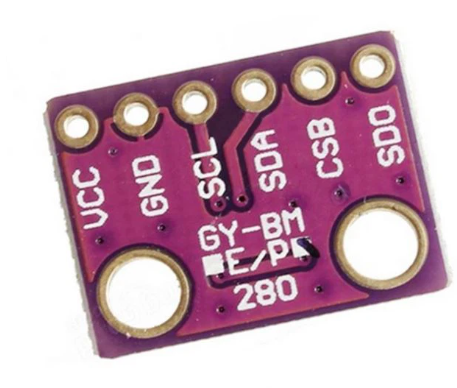
\includegraphics[width=0.8\linewidth]{gambar/Dasar teori/Sensor BME280.png}
			\caption{Sensor BME280}
			\label{gambar1}
		\end{figure}
		
		\item Menentukan rentang nilai yang akan dijadikan data dummy dengan merujuk pada penelitian yang membahas mengenai implementasi sensor BME280 pada studi kasus pengukuran stasiun cuaca dalam 3 hari berturut-turut. Mengacu pada penelitian tersebut, rentang data yang dihasilkan sensor dalam 10 detik berkisar sekitar 28,47℃ - 34,46 ℃ untuk suhu, 50,78\% - 59,17\% untuk kelembaban, 1008,27 hPa - 1009,24 hPa untuk tekanan udara, dan 40,14 - 63,67 m untuk ketinggian [15]. 
		
		\item Membuat file berformat Python dengan nama sensor-data.py.
		\item Menginstal Flask dengan perintah “pip install flask-cors”. Flask merupakan salah satu framework Python yang ringan dan mudah dikustomisasi serta dapat dimanfaatkan dalam pengembangan website. Flask menyediakan fitur yang dapat disesuaikan dengan kebutuhan pengembang tanpa harus berpatokan dengan standar atau struktur sebuah framework [35]. Pada konteks ini, Flask dimanfaatkan sebagai framework untuk pembuatan data API dummy yang akan digunakan untuk pengujian. Alasan pemilihan framework ini adalah karena ukurannya yang kecil dan fleksibilitasnya sehingga tidak membebani memori serta dapat dikonfigurasi dengan mudah. 
		\begin{figure}[H]
			\centering
			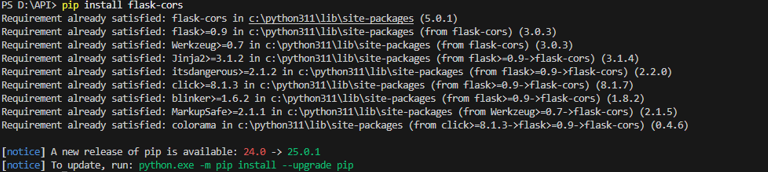
\includegraphics[width=0.8\linewidth]{gambar/Dasar teori/Flask.png}
			\caption{Install Flask}
			\label{Instal Flask}
		\end{figure}
		
		\item Menerapkan beberapa library, seperti berikut : 
		\begin{figure}[H]
			\centering
			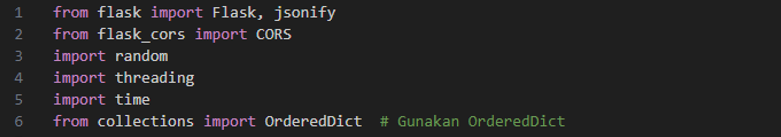
\includegraphics[width=0.8\linewidth]{gambar/Dasar teori/Library.png}
			\caption{Library}
			\label{Menambahkan Library}
		\end{figure}
		\begin{enumerate}[label={\alph*.}]
			\item jsonify: Mengubah data menjadi format JSON untuk dikirim ke client.
			\item CORS: Mengizinkan permintaan dari domain berbeda (Cross-Origin Resource Sharing). Digunakan untuk menghubungkan port 5000 dari python dan port 8000 dari HTTP. 
			\item random: Digunakan untuk menghasilkan data acak untuk membuat simulasi sensor. 
			\item threading: Digunakan untuk menjalankan fungsi secara paralel memperbarui data sensor secara terus-menerus.
			\item time: Mengatur delay dalam proses pembaruan data.
		\end{enumerate}
		
		\item Inisialisasi Flask dan Konfigurasi CORS
		\begin{figure}[H]
			\centering
			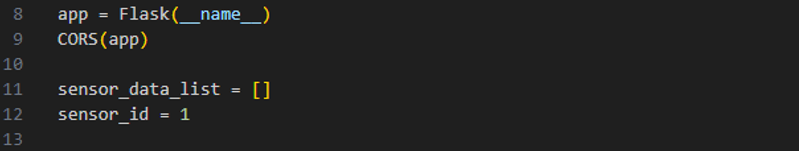
\includegraphics[width=0.8\linewidth]{gambar/Dasar teori/Initiate.png}
			\caption{Inisialisasi Flask dan CORS}
			\label{Inisialisasi Flask dan CORS}
		\end{figure}
		
		\item Variabel sensor\_data\_list digunakan untuk menyimpan data sensor yang terus diperbarui.
		\begin{figure}[H]
			\centering
			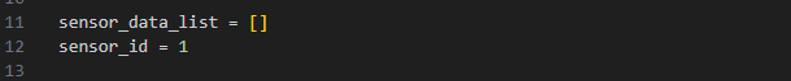
\includegraphics[width=0.8\linewidth]{gambar/Dasar teori/variabel.png}
			\caption{variabel}
			\label{Inisialisasi Variabel}
		\end{figure}
		
		\item Membuat fungsi untuk membuat data sensor yang menghasilkan dan menyimpan data setiap 10 detik dalam rentang data 28.47℃ - 34.53℃ untuk suhu, 59.13\% - 50.78\% untuk humidity, 1008 hPa - 1011 hPa untuk pressure, dan 40.16 m - 63.67m untuk altitude. Sensor ini dibuat untuk terus me-looping pembuatan data dengan struktur: 
		\begin{enumerate}[label={\alph*.}]
			\item Id nilai unik untuk mengidentifikasi data 
			\item Timestamp dalam format standar ISO 8601
			\item Temperature dalam satuan derajat celcius hingga derajat celcius 
			\item Humidity dalam satuan RH
			\item Pressure dalam satuan HPa 
			\item Altitude dalam satuan meter
		\end{enumerate}
		\begin{figure}[H]
			\centering
			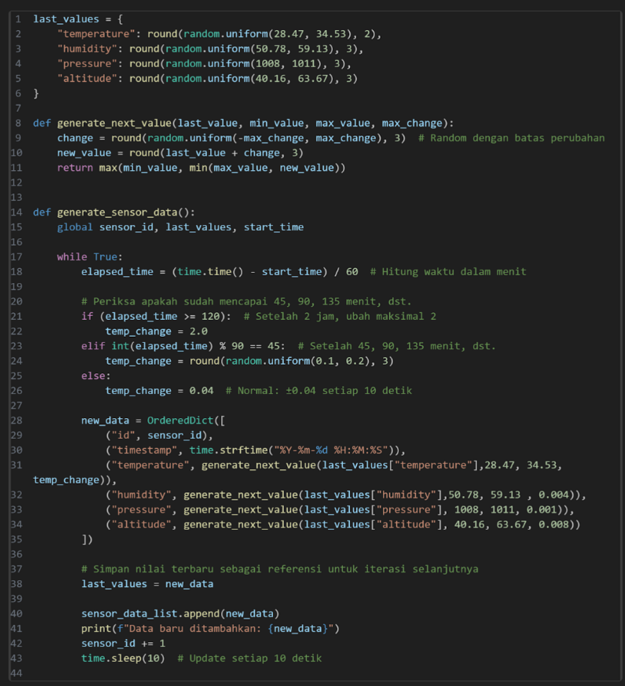
\includegraphics[width=0.8\linewidth]{gambar/Dasar teori/generate_dummy.png}
			\caption{Membuat Sensor Dummy}
			\label{Membuat Sensor Dummy}
		\end{figure}
		
		\item Membuat API Endpoint. API endpoint ini akan digunakan untuk mengambil data dan mengurutkannya dalam format JSON dengan library jsonify.
		\begin{figure}[H]
			\centering
			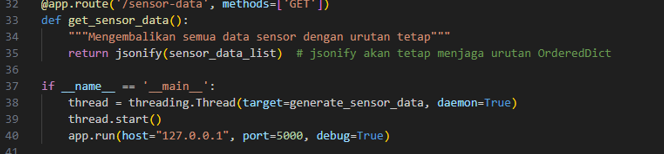
\includegraphics[width=0.8\linewidth]{gambar/Dasar teori/API.png}
			\caption{API Endpoint}
			\label{API Endpoint}
		\end{figure}
		
		\item Menjalankan program threading pada fungsi generate\_sensor\_data secara berkala, paralel dengan server Flask untuk menangani request.
		\begin{figure}[H]
			\centering
			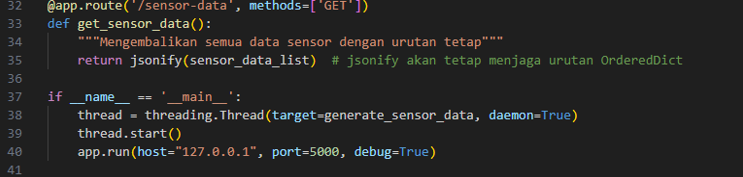
\includegraphics[width=0.8\linewidth]{gambar/Dasar teori/threading.png}
			\caption{Menjalankan Program Threading}
			\label{Menjalankan Program Threading}
		\end{figure} 
		
		\item Menjalankan server tersebut dengan “python sensor-data.py”. 
		\begin{figure}[H]
			\centering
			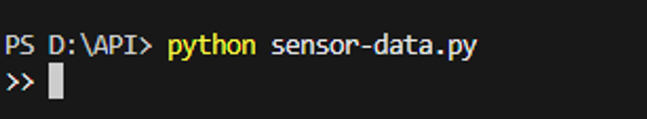
\includegraphics[width=0.8\linewidth]{gambar/Dasar teori/Run.png}
			\caption{Menjalankan Sensor}
			\label{Menjalankan Sensor}
		\end{figure}
	\end{enumerate}
	\item Multiple Sensor \\
	Data yang dijadikan acuan sebagai contoh data yang mengintegrasikan beberapa sensor pengukuran adalah data yang merujuk pada jurnal “A Comprehensive IoT edge based smart irrigation system for tomato cultivation” [33]. Berdasarkan data yang diperoleh dari jurnal tersebut, struktur json yang ditampilkan adalah sebagai berikut :
	\pagebreak
	\begin{longtable}{|p{.35\linewidth}|p{.60\linewidth}|}
		\caption{Struktur JSON dari Sensor}
		\label{tab:json_sensor} \\  
		\hline
		\multicolumn{2}{|l|}{\textbf{Struktur JSON:}} \\ \hline
		\multicolumn{2}{|c|}{%
			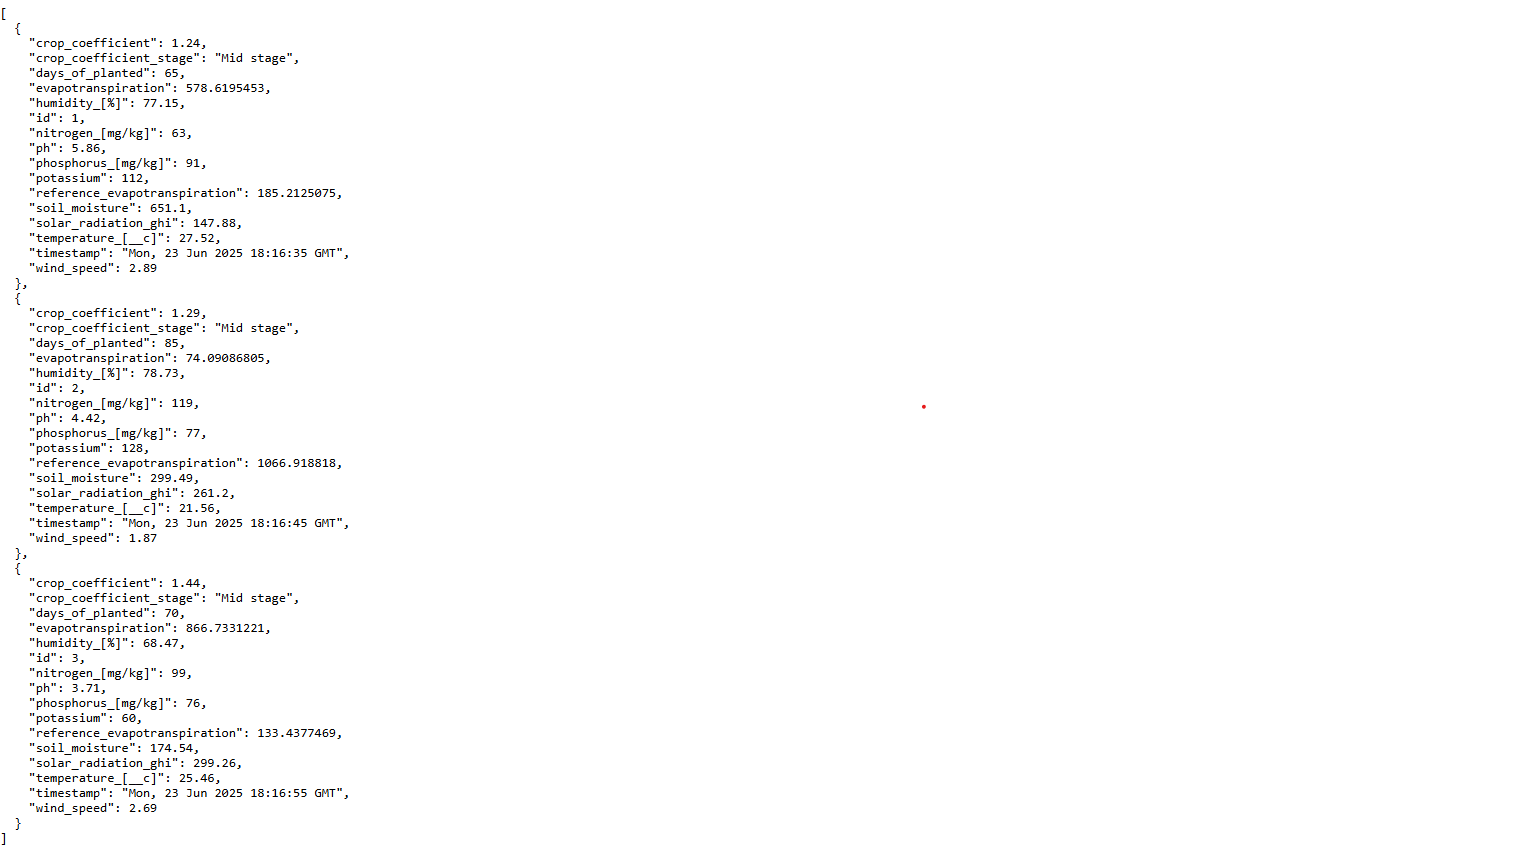
\includegraphics[width=0.8\linewidth, margin=5pt 10pt 5pt 10pt ]{gambar/Metodologi/StrukturJSON2.png}
		} \\ \hline
		\textbf{Parameter} & \textbf{Keterangan} \\ \hline
		\texttt{crop\_coefficient} & Koefisien tanaman (Kc) menggambarkan kebutuhan air relatif tanaman pada fase pertumbuhan tertentu \\ \hline
		\texttt{crop\_coefficient\_stage} & Tahapan pertumbuhan tanaman saat ini \\ \hline
		\texttt{days\_of\_planted} & Hari sejak tanaman ditanam \\ \hline
		\texttt{evapotranspitarion} & Jumlah air yang hilang akibat penguapan \\ \hline
		\texttt{humidity} & Kelembapan udara \\ \hline
		\texttt{nitrogen} & Kandungan nitrogen pada tanah \\ \hline
		\texttt{ph} & Tingkat keasaman tanah \\ \hline
		\texttt{phosphorus} & Kandungan fosfor pada tanah \\ \hline
		\texttt{potassium} & Kandungan kalium di dalam tanah \\ \hline
		\texttt{reference\_evaporation} & nilai standar berdasarkan tanaman acuan\\ \hline
		\texttt{soil\_mosture} & kelembapan tanah \\ \hline
		\texttt{solar\_radiation\_ghi} & Radiasi\\ \hline
		\texttt{temperature} & Suhu udara saat pengukuran \\ \hline
		\texttt{timestamp} & Waktu saat data diambil \\ \hline
		\texttt{windspeed} & Kecepatan angin \\ \hline
	\end{longtable}
	Tahapan yang dilakukan dalam menampilkan data tersebut menjadi data real-time yang siap uji antara lain : 
	\begin{enumerate}[label={\arabic*.}]
		\item Mengunduh sumber data hasil pengukuran dalam bentuk csv. 
		\item Memanfaatkan framework Flask untuk menampilkan data tersebut dan menggunakan library pandas untuk mengolah data csv.
		\item Melakukan data preprocessing dengan mengubah semua huruf menjadi huruf kecil, mengganti spasi dengan underscore agar mudah dipahami, serta melakukan teknik oversampling pada data agar data bertambah dari jumlah data aslinya. Teknik oversampling adalah teknik untuk menambahkan data dari kelas minoritas ke dalam data pelatihan secara acak. Penambahan ini dilakukan berulang-ulang hingga jumlah data pada kelas minoritas setara dengan jumlah data pada kelas mayoritas [36]
		\begin{figure}[H]
			\centering
			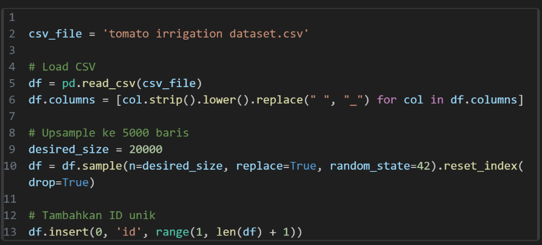
\includegraphics[width=0.8\linewidth]{gambar/Metodologi/Mount_preprocessing.png}
			\caption{Mounting Data}
			\label{Mounting Data}
		\end{figure}
		\item Membuat kolom timestamp agar dapat menampilkan data secara realtime selama pengujian. 
		\begin{figure}[H]
	\centering
	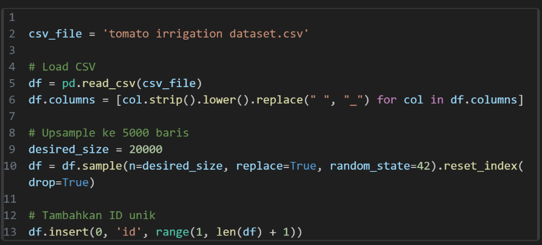
\includegraphics[width=0.8\linewidth]{gambar/Metodologi/kolom_timestamp.png}
	\caption{Membuat kolom timestamp}
	\label{Membuat Timestamp Data}
\end{figure}
		\item Membuat endpoint untuk mengambil data sensor dan menambahkan data ke dalam json setiap 10 detik. Data akan terus menerus digenerate seperti ketika sensor mengambil data real-time dari aplikasi. 
		\begin{figure}[H]
			\centering
			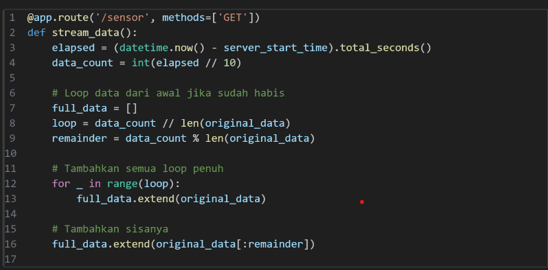
\includegraphics[width=0.8\linewidth]{gambar/Metodologi/endpoint.png}
			\caption{Membuat Endpoint API}
			\label{Membuat Endpoint}
		\end{figure}
		\item Menjalankan server Flask dalam mode debug untuk mempermudah pengembangan karena auto-reload dan error ditampilkan.
		\begin{figure}[H]
			\centering
			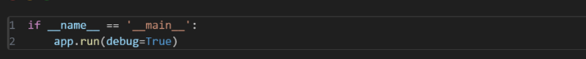
\includegraphics[width=0.8\linewidth]{gambar/Metodologi/run.png}
			\caption{Menjalankan Server}
			\label{Menjalankan Server}
		\end{figure}
		
	\end{enumerate}
\end{enumerate}

\section{Alat}
Salah satu tujuan penelitian ini adalah untuk meninjau performa rendering dan penggunaan resource pada perangkat saat melakukan visualisasi data dari perangkat sensor IoT. Oleh karena itu, penelitian ini membutuhkan peralatan software dan hardware untuk menunjang penelitian.
\subsection{Perangkat Lunak}
Peralatan perangkat lunak yang digunakan dalam pengembangan sistem ini, meliputi sistem operasi, library, dan aplikasi yang digunakan, yang dijelaskan sebagai berikut :  

\begin{longtable}{|p{\dimexpr.35\linewidth-2\tabcolsep-1.25\arrayrulewidth}|
		p{\dimexpr.20\linewidth-2\tabcolsep-1.25\arrayrulewidth}|
		p{\dimexpr.45\linewidth-2\tabcolsep-1.25\arrayrulewidth}|}
	\caption{Spesifikasi Perangkat Lunak} \label{t_risetPemodelan} \\
	
	\hline
	\textbf{Nama Perangkat Lunak} & \textbf{\textit{Versi}} & \textbf{Keterangan} \\ \hline
	\endfirsthead
	
	\hline
	\textbf{Nama Perangkat Lunak} & \textbf{\textit{Versi}} & \textbf{Keterangan} \\ \hline
	\endhead
	
	\hline \multicolumn{3}{r}{{Lanjut ke halaman berikutnya}} \\ 
	\endfoot
	
	\hline
	\endlastfoot
	
	Visual Studio Code & 1.97.0 & Digunakan untuk membuat \textit{website}, dari segi \textit{Frontend} dan \textit{Backend}. \\ \hline
	
	Python & 3.11.4 & Digunakan untuk membuat data \textit{dummy} guna menguji cobakan \textit{chart} visualisasi. \\ \hline
	
	Chart.js & 4.0 & \textit{Versi} Chart.js saat diuji cobakan. Digunakan untuk membuat visualisasi. \\ \hline
	
	D3.js & 7.9.0 & \textit{Versi} D3.js saat diuji cobakan. Digunakan untuk membuat visualisasi. \\ \hline
	
	Highcharts & 12.1.2 & \textit{Versi} Highcharts saat diuji cobakan. Digunakan untuk membuat visualisasi. \\ \hline
	
\end{longtable}


\subsection{Perangkat Keras}
Peralatan perangkat keras yang digunakan dalam pengembangan sistem ini, meliputi spesifikasi laptop yang digunakan untuk mengembangkan dan menjalankan website, yang dijelaskan sebagai berikut :  

\begin{table}[h!]
	\centering
	\renewcommand{\arraystretch}{1.5} % jarak baris lebih renggang
	\caption{\textit{Spesifikasi Perangkat Keras yang Digunakan}}
	\label{tab:spesifikasi_perangkat_keras}
	\begin{tabular}{|>{\raggedright\arraybackslash}p{4cm} 
			|>{\raggedright\arraybackslash}p{8cm}|}
		\hline
		\textbf{Spesifikasi} & \textbf{Keterangan} \\
		\hline
		Operating System & Windows 11 64-bit \\
		\hline
		Processor & Intel(R) Core (TM) i5-10300H \\
		\hline
		CPU & 2.5 GHz \\
		\hline
		Memory & 8GB DDR4 SO-DIMM 2666MHz \\
		\hline
		Graphic & NVIDIA\textregistered~GeForce\textregistered~GTX 1650 4GB GDDR6 \\
		\hline
	\end{tabular}
\end{table}


\section{Tahapan Proyek Akhir}
Dalam penelitian yang berjudul Analisis Perbandingan Kinerja Library Chart.js, Highcharts, dan D3.js untuk Visualisasi Data Sensor IoT pada Dashboard Berbasis Laravel, penulis melalui beberapa tahapan penting untuk mendapatkan hasil yang komprehensif. Tahapan pertama adalah fase studi literatur, selanjutnya adalah pengembangan website, di mana penulis membangun sebuah dashboard berbasis Laravel yang mampu menampilkan data sensor IoT secara dinamis. Setelah itu, pada fase implementasi library, tiga library visualisasi Chart.js, Highcharts, dan D3.js diimplementasikan ke dalam sistem untuk menampilkan data dalam format grafik line chart. Tahapan terakhir adalah fase komparasi, yang bertujuan untuk mengevaluasi kinerja masing-masing library berdasarkan berbagai parameter yang telah ditentukan sebelumnya. Melalui pendekatan ini, penelitian diharapkan dapat memberikan wawasan mendalam mengenai library yang paling optimal untuk memvisualisasikan data IoT. Alur penelitian ini dijelaskan dalam bagan berikut : 

\begin{figure}[H]
	\centering
	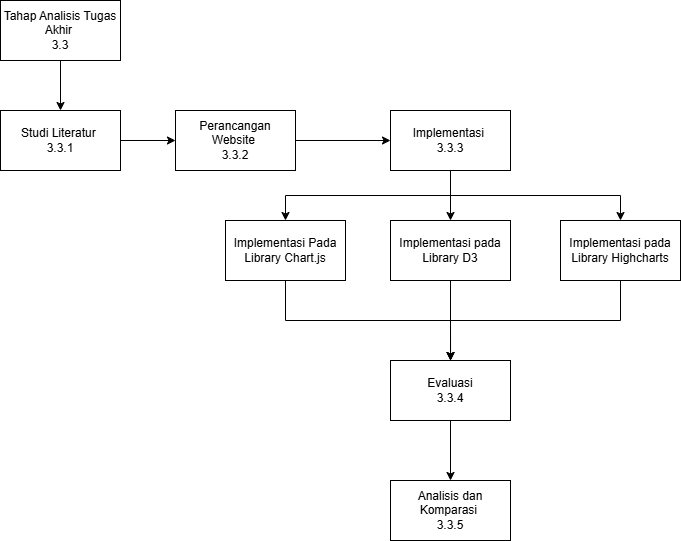
\includegraphics[width=0.8\linewidth]{gambar/Metodologi/Alur penelitian.png}
	\caption{Alur Penelitian}
	\label{Alur Penelitian}
\end{figure}

\subsection{Studi Literatur}
Tahap ini dilakukan untuk memperoleh landasan yang mendukung pelaksanaan penelitian. Literatur yang dikaji mencakup teori-teori utama yang relevan dengan topik, serta penelitian terdahulu yang berkaitan dengan pendekatan dan metode yang digunakan dalam penelitian ini. 

Penelitian dilakukan dengan menggunakan metode eksperimen dengan pendekatan kuantitatif. Pendekatan ini dilakukan secara runtut dan rasional, di mana peneliti secara langsung mengatur variabel bebas untuk melihat dampaknya terhadap variabel yang dipengaruhi, dalam situasi yang telah dikendalikan. Dengan metode ini, peneliti memiliki kontrol atas variabel bebas baik sebelum maupun saat proses eksperimen berlangsung. Proses ini juga disertai dengan pengukuran data secara kuantitatif guna mengetahui adanya hubungan sebab dan akibat antara variabel yang diteliti. Tujuan dari pendekatan ini adalah untuk menguji kebenaran hipotesis yang telah dirumuskan, memperkirakan hasil dari perlakuan yang diberikan, serta menyimpulkan pola hubungan antar variabel secara umum [37]. Dalam konteks ini, variabel bebas yang dimaksud adalah Chart.js, D3, dan Highcharts, serta variabel terikat adalah waktu render, penggunaan CPU, dan penggunaan memori.

Terdapat beberapa studi literatur yang digunakan sebagai acuan pengukuran dalam penelitian ini. Berdasarkan rujukan jurnal yang dijelaskan pada bab sebelumnya, waktu rendering, penggunaan memori, dan alokasi CPU seringkali dijadikan sebagai indikator pengukuran performa suatu website visualisasi karena ketiganya memengaruhi alokasi sumber daya (resources) pada sistem komputer yang menentukan pengalaman pengguna (user experience) dan efisiensi sistem [3], [4], [35].

Berdasarkan rujukan yang digunakan, indikator tersebut berbanding lurus dan saling mempengaruhi satu sama lain. Peningkatan pada satu indikator cenderung diikuti oleh peningkatan pada indikator lainnya. Misalnya, karena kompleksitas visualisasi yang tinggi atau penggunaan fitur interaktif yang intensif, maka penggunaan memori juga akan bertambah untuk menyimpan elemen visual serta data yang ditampilkan. Korelasi ini menjadi penting untuk dianalisis secara menyeluruh guna memahami performa sistem secara holistik. Fitur-fitur utama dari visualisasi data seperti interaktivitas, kompleksitas elemen grafik, jumlah data yang divisualisasikan, serta kemampuan dukungan real-time sangat memengaruhi performa render. Semakin tinggi tingkat interaktivitas serta semakin kompleks grafik, maka semakin besar pula beban terhadap CPU dan memori sistem, serta semakin lama waktu yang dibutuhkan untuk menampilkan visualisasi secara utuh. Merujuk pada website dari Chart.js [5], D3.js [6], dan Highcharts [7], perbandingan yang ditinjau dari aspek yang telah disebutkan dijelaskan seperti pada tabel berikut :
\begin{table}[H]
	\centering
	\renewcommand{\arraystretch}{1.5} % jarak baris lebih renggang
	\caption{Perbandingan Chart.js, D3.js, dan Highcharts}
	\label{tab:perbandingan_library}
	\begin{tabular}{|>{\raggedright\arraybackslash}p{3.5cm}
			|>{\raggedright\arraybackslash}p{3.5cm}
			|>{\raggedright\arraybackslash}p{3.5cm}
			|>{\raggedright\arraybackslash}p{3.5cm}|}
		\hline
		\rowcolor[gray]{0.85}
		\textbf{Aspek} & \textbf{Chart.js} & \textbf{D3.js} & \textbf{Highcharts} \\
		\hline
		Ketersediaan \textit{open source} 
		& Tersedia 
		& Tersedia 
		& Tersedia \\ 
		\hline
		Dukungan Interaktif 
		& Mendukung interaktivitas seperti \textit{tooltip}, \textit{zoom}, dan \textit{hover}. 
		& Interaksi kompleks termasuk \textit{tooltip}, \textit{zoom}, dan animasi.
		& Interaktif dengan built-in fitur \textit{tooltip}, \textit{drilldown}, \textit{zoom}, \textit{pan}, dan animasi. \\
		\hline
		Basis grafik 
		& Menggunakan Canvas 
		& Menggunakan SVG atau Canvas 
		& Menggunakan SVG (default) \\
		\hline
		Dukungan data \textit{real-time} 
		& Didukung dengan update dinamis menggunakan \texttt{chart.update()} 
		& Harus dikodekan manual 
		& Mendukung data \textit{real-time} dengan fitur bawaan \texttt{setData()} \\
		\hline
	\end{tabular}
\end{table}

\subsection{Perancangan Website}
Dalam prosesnya, pengembangan website ini dibagi menjadi dua bagian utama, yaitu Frontend dan Backend. Frontend merupakan sisi pengembangan yang berfokus pada tampilan dan interaksi pengguna. Sementara Backend menangani manajemen database dan API. Penelitian ini secara khusus berfokus pada pengembangan Frontend yang mencakup implementasi desain serta analisis penggunaan Library visualisasi. Proses pengembangan Frontend melibatkan berbagai teknologi seperti HTML, CSS, dan JavaScript. Dengan fokus pada Frontend, penelitian ini bertujuan untuk menghasilkan tampilan website yang responsif dan mudah digunakan oleh pengguna. Adapun aspek Backend yang berhubungan dengan manajemen data dan logika pemrosesan tidak dibahas dalam penelitian ini, sehingga integrasi dengan sistem Backend akan menjadi pertimbangan dalam implementasi lanjutan.

\subsubsection{Perancangan Desain Sistem}
Selain data uji, diperlukan pula perancangan sistem yang menjadi bahan untuk mendefinisikan struktur, alur kerja, dan interaksi sistem sebelum tahap implementasi dilakukan. Pada tahap ini, diperlukan pendefinisian kebutuhan, use case diagram dan sequence diagram, serta kebutuhan data pengujian. Kebutuhan fungsional yang dimaksud mencakup fitur-fitur utama yang harus ada dalam sistem agar sesuai dengan tujuan. Berikut adalah beberapa kebutuhan fungsional dalam website yang menampilkan data IoT:

\begin{enumerate}[label={\arabic*.}]
	\item Website harus mampu mengambil data secara real-time melalui API.
	\item Website mampu menambahkan lebih dari satu visualisasi dengan dukungan terhadap jenis grafik seperti line chart, bar chart, dan scatter plot. 
\end{enumerate}

Sedangkan kebutuhan non-fungsional yang dimaksud, berkaitan dengan kualitas sistem dan aspek teknis yang memastikan website berjalan dengan optimal. Kebutuhan tersebut meliputi: 
\begin{enumerate}[label={\arabic*.}]
	\item Sistem mampu menangani volume data besar yang terus bertambah dari perangkat IoT.
	\item Kode terdokumentasi dengan baik, sehingga mudah diperbarui atau diperbaiki.
\end{enumerate}

Untuk mengimplementasi kebutuhan fungsional dan non fungsional, diagram yang dibutuhkan antara lain adalah use case diagram dan sequence diagram. Use Case Diagram adalah diagram Unified Modeling Language (UML) yang menggambarkan interaksi antara pengguna (actors) dengan sistem melalui berbagai fitur penggunaan (use cases). Use case diagram dapat membantu pengembang akan lebih mudah dalam melakukan analisis kebutuhan, serta merancang fitur yang akan dikembangkan. Pada sistem yang sedang diteliti, use case diagram berikut menggambarkan fitur-fitur yang berkaitan dengan penelitian, seperti gambar berikut :

\begin{figure}[H]
	\centering
	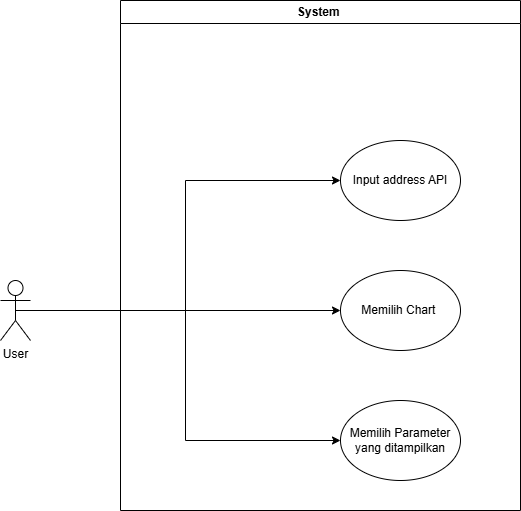
\includegraphics[width=0.8\linewidth]{gambar/Metodologi/Use Case.png}
	\caption{use Case Diagram}
	\label{Use Case Diagram}
\end{figure}

Sequence Diagram merupakan diagram UML yang digunakan untuk menggambarkan bagaimana objek berinteraksi dan bertukar pesan seiring waktu. Diagram ini menunjukkan bagaimana pesan dikirim antara objek atau instance lainnya untuk menyelesaikan suatu tugas. Sequence Diagram digunakan pada tahap perancangan detail, dimana komunikasi antar proses harus ditetapkan secara tepat [39].  Sequence Diagram untuk website ini digambarkan seperti berikut :

\begin{figure}[H]
	\centering
	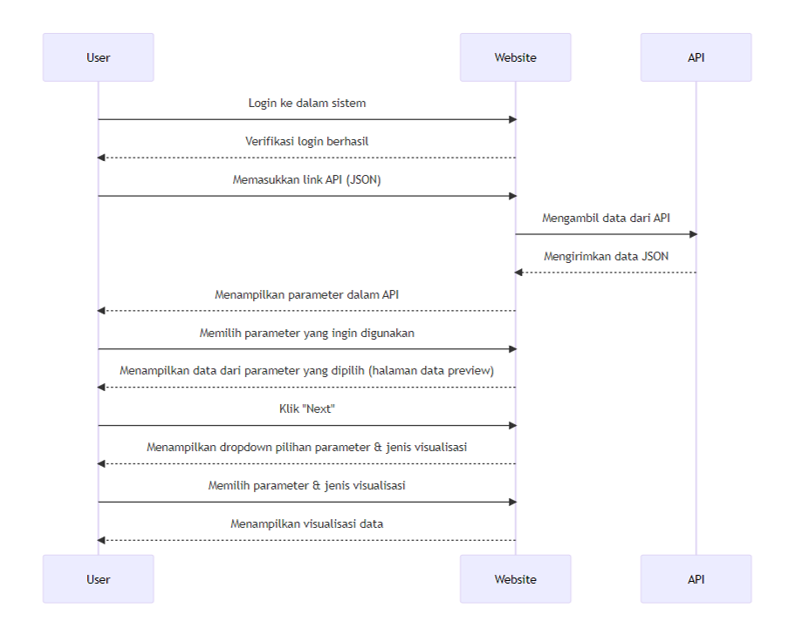
\includegraphics[width=0.8\linewidth]{gambar/Metodologi/Sequence Diagram.png}
	\caption{Sequence Diagram}
	\label{Sequence Diagram}
\end{figure}

\subsubsection{Perancangan UI}
Sebelum tahap pengembangan frontend, diperlukan perancangan User Interface dengan Figma yang akan digunakan sebagai acuan untuk membuat kode Frontend, rancangan user interface tersebut dibagi menjadi dua halaman utama dan 3 komponen tambahan, seperti berikut : 
\begin{enumerate}[label={\arabic*.}]
	\item Halaman Utama \\
	Halaman ini merupakan halaman pertama yang akan dilihat pengguna setelah mengakses website. Pada bagian ini, pengguna dapat menginputkan API dari data IoT pada field input yang tersedia, kemudian setelah di klik generate, parameter pada API tersebut akan tertampil dalam bentuk checkbox. 
	\begin{figure}[H]
		\centering
		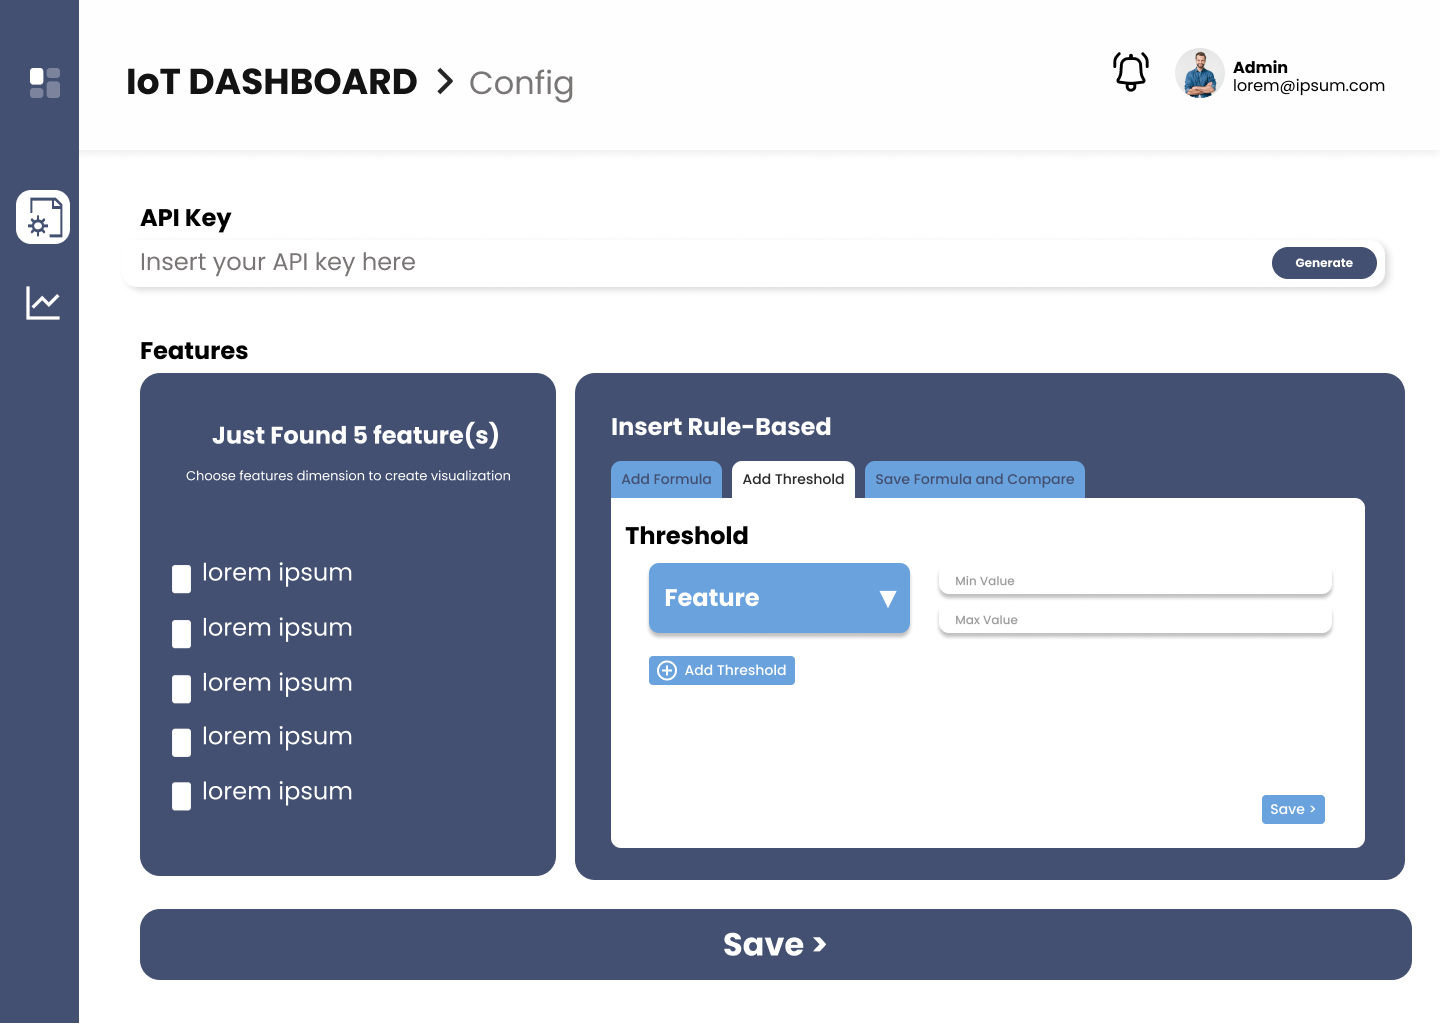
\includegraphics[width=0.8\linewidth]{gambar/Metodologi/main.png}
		\caption{Halaman Utama}
		\label{Halaman Utama}
	\end{figure}
	Adapun fitur yang ada di dalam halaman ini adalah kolom input alamat API untuk menginputkan alamat API dari pengguna, Checkbox untuk menampilkan parameter yang ada di dalam API, Tab rules untuk memberikan pengaturan terhadap data-data yang masuk. Seperti mengatur ambang batas, formula, dan komparasi formula. 
	\item Formula \\
	Merupakan fitur yang digunakan untuk menyimpan rumus tertentu yang dapat difungsikan sebagai threshold atau alert saat data menyentuh suatu titik tertentu yang dianggap tidak wajar. 
	\begin{figure}[H]
		\centering
		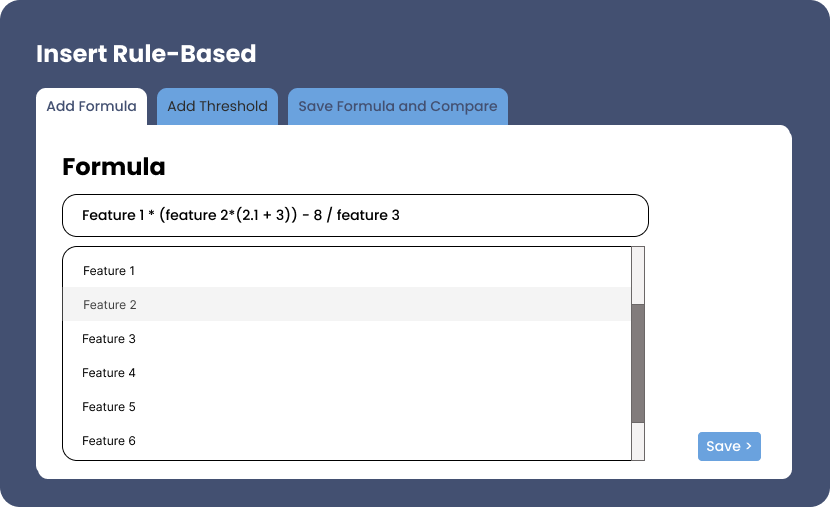
\includegraphics[width=0.8\linewidth]{gambar/Metodologi/formula.png}
		\caption{Menambahkan Formula}
		\label{gambar1}
	\end{figure}
	\item Threshold\\
	 Merupakan fitur yang digunakan untuk menyimpan ambang batas minimal dan maksimal dari suatu fitur data sehingga sistem akan memunculkan peringatan ketika data melampaui ambang batas. 
	 \begin{figure}[H]
	 	\centering
		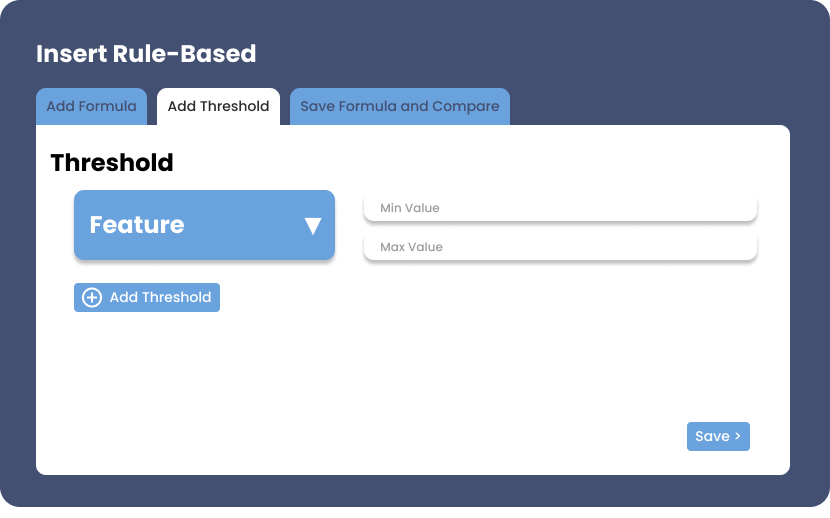
\includegraphics[width=0.8\linewidth]{gambar/Metodologi/threshold.png}
	 	\caption{Menambahkan Ambang Batas}
	 	\label{Menambahkan Ambang Batas}
	 \end{figure}
	 \item Save Formula and Compare\\
	 Digunakan untuk membandingkan antara threshold dan batasan tertentu. Sehingga ketika terdapat perbedaan, maka sistem akan menampilkan alert. Pada tab ini, pengguna dapat memilih dua fitur untuk dibandingkan. 
	 	 \begin{figure}[H]
	 	\centering
	 	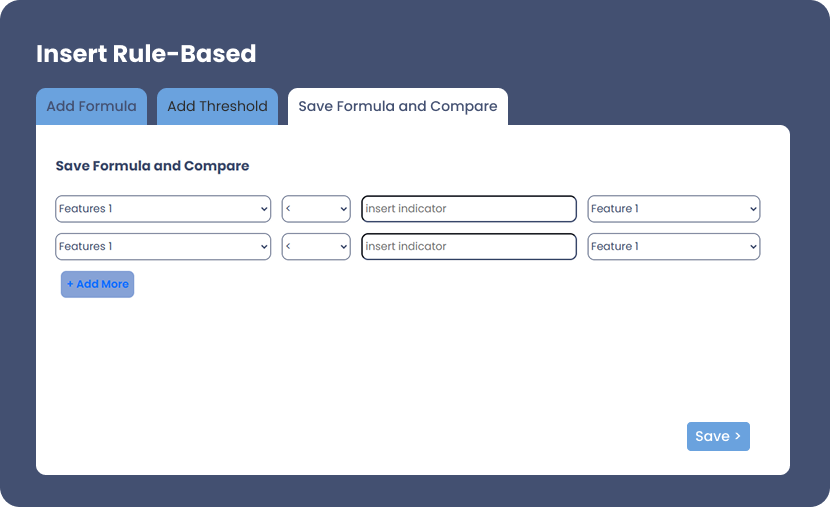
\includegraphics[width=0.8\linewidth]{gambar/Metodologi/compare.png}
	 	\caption{Menambahkan Ambang Batas}
	 	\label{Menambahkan Ambang Batas}
	 \end{figure}
	 \item Halaman visualisasi dan Chart\\
	 Halaman ini digunakan untuk memvisualisasikan perbandingan dari suatu fitur dengan fitur lainnya melalui bar chart, line chart, dan scatter plot.
	 	 \begin{figure}[H]
	 	\centering
	 	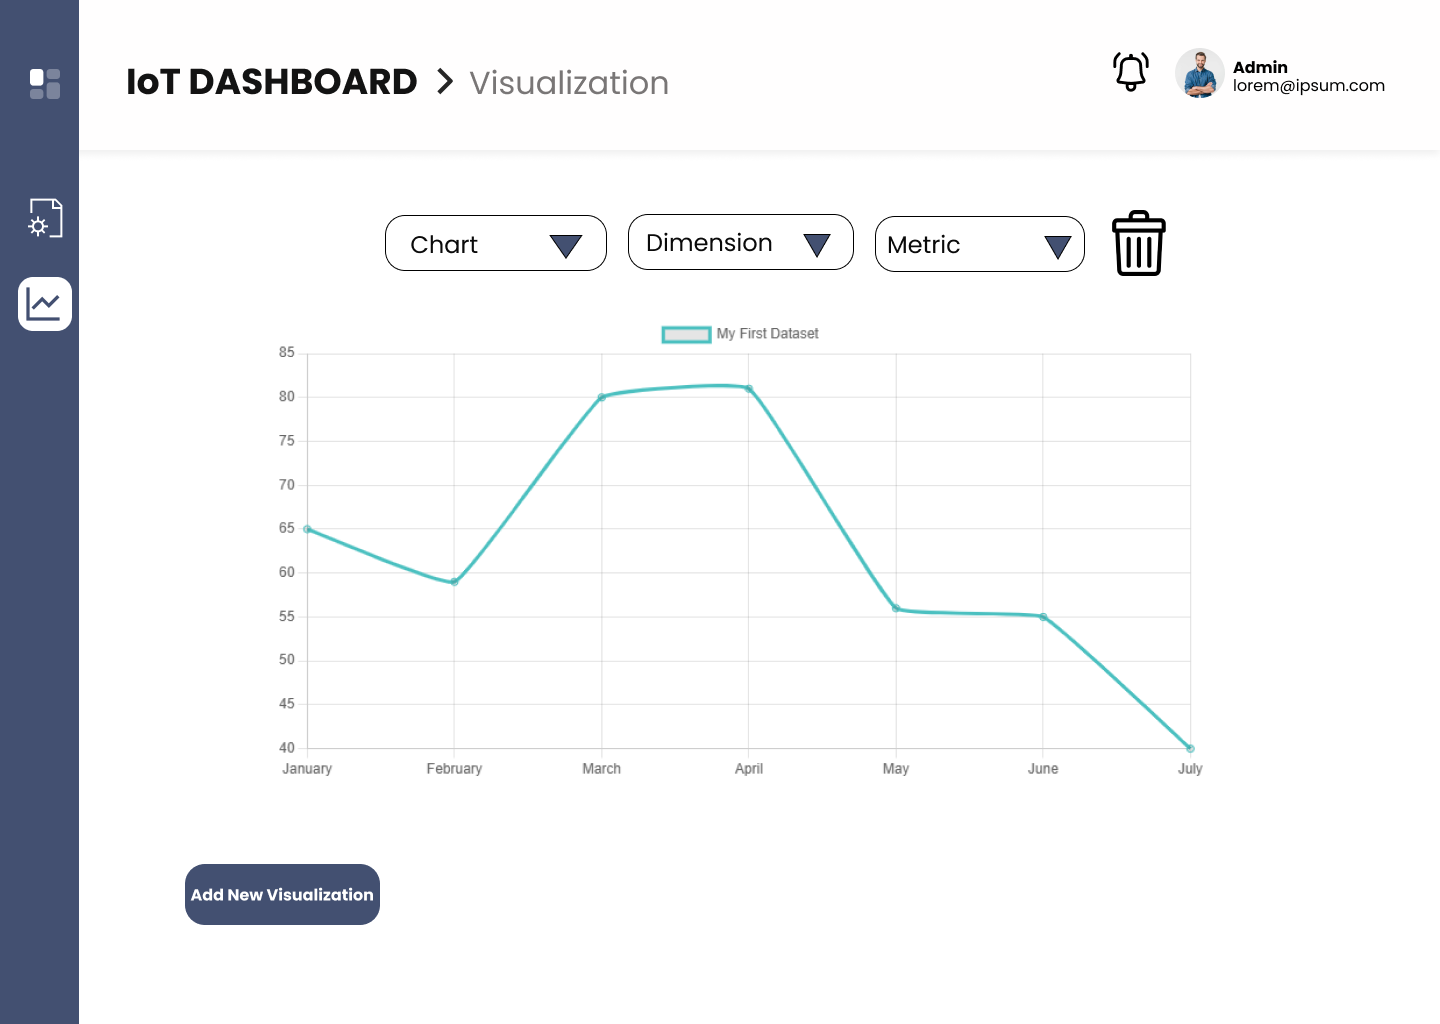
\includegraphics[width=0.8\linewidth]{gambar/Metodologi/visualization page.png}
	 	\caption{Menambahkan Ambang Batas}
	 	\label{Menambahkan Ambang Batas}
	 \end{figure} 
\end{enumerate}
\subsection{Implementasi}
Setelah menyiapkan data, maka tahap selanjutnya adalah tahap implementasi. Tahap ini akan menjelaskan implementasi Chart.js, D3.js, dan Highcharts dalam menampilkan visualisasi. Implementasi dilakukan dengan menggunakan skrip Javascript yang sama dengan penyesuaian pada bagian fungsi createChart() sesuai dengan library JavaScript yang digunakan. Fungsi-fungsi lain yang digunakan dalam tahap ini telah dijelaskan pada sub-bab “Pembuatan Website”. 

\subsection{Evaluasi}
Proses ini bertujuan untuk mengetahui perbedaan signifikan dalam waktu rendering, efisiensi pengolahan data visual, serta kemampuan masing-masing library dalam menangani beban visualisasi yang berbeda. Dalam prosesnya, semua pengujian dilakukan dalam lingkungan hardware, software, dan versi browser yang sama serta kondisi browser selalu dipastikan bersih sebelum melakukan pengujian lainnya dengan selalu memulai ulang kondisi browser. Dengan melakukan perbandingan ini, diharapkan dapat ditemukan library yang paling optimal dan sesuai untuk digunakan dalam pengembangan sistem visualisasi data. Setelah diimplementasikan, performa akan dievaluasi berdasarkan parameter-parameter yang telah ditentukan, meliputi : 
\begin{enumerate}
	\item Performa rendering

	Performa akan diukur dengan fungsi bawaan dari Javascript [3], [4]. Pengukuran dilakukan dengan memanfaatkan fungsi dari JavaScript console.time() dan performance.now() yang ditempatkan di dalam fungsi createChart() untuk mengukur waktu render. Fungsi performance.now() adalah fungsi di JavaScript yang digunakan untuk mengukur waktu secara presisi sehingga dapat digunakan untuk mengetahui durasi eksekusi suatu proses dalam aplikasi web [40]. Pengukuran ini dilakukan dengan tahapan : 
	\begin{enumerate}[label={\arabic*.}]
		\item menjalankan server data dummy dan server website secara lokal,
		\item menampilkan visualisasi pada website, 
		\item meninjau waktu render melalui file berformat .txt yang telah otomatis di-generate dari console menggunakan fungsi performance.now() yang memberikan nilai waktu relatif, yaitu berapa milidetik yang dihitung sejak fungsi dijalankan. 
			\begin{figure}[H]
			\centering
			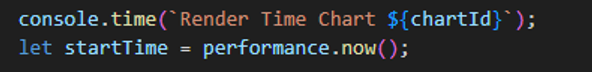
\includegraphics[width=0.8\linewidth]{gambar/Metodologi/Start Performance Now.png}
			\caption{Mulai Pengukuran}
			\label{Mulai Pengukuran Render}
		\end{figure}
			\begin{figure}[H]
			\centering
			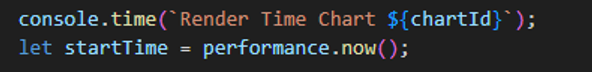
\includegraphics[width=0.8\linewidth]{gambar/Metodologi/Start Performance Now.png}
			\caption{Akhir Pengukuran}
			\label{Akhir Pengukuran Render}
		\end{figure}
	\end{enumerate}
			Setelah seluruh proses selesai dijalankan dan waktu render telah terekam, data tersebut akan digunakan untuk menghitung rata-rata waktu render di setiap titik yang telah ditentukan. Nilai rata-rata ini berperan penting dalam proses evaluasi, karena mampu mereduksi pengaruh noise atau outlier yang mungkin muncul selama pengujian. Dengan demikian, pengukuran performa website menjadi lebih stabil, representatif, dan dapat mencerminkan tingkat skalabilitas sistem secara lebih akurat.
	
	\item Alokasi Footprint Memory 
	
	Pengukuran penggunaan memori dilakukan dengan memanfaatkan fitur Chrome Task Manager, dengan cara mencatat nilai Memory Footprint pada tab Chrome tertentu. Nilai ini menggambarkan total memori yang digunakan oleh tab tersebut, mencakup memori yang dipakai untuk proses rendering halaman, eksekusi skrip JavaScript, serta pemuatan berbagai sumber daya yang ada di dalam halaman web. Pendekatan ini membantu memperoleh perkiraan konsumsi memori yang lebih terfokus pada aktivitas halaman yang diuji.
		\begin{figure}[H]
		\centering
		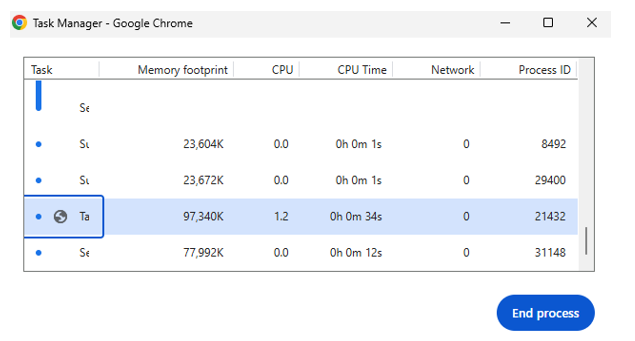
\includegraphics[width=0.8\linewidth]{gambar/Metodologi/Task Manager.png}
		\caption{Pengukuran Footprint Memory}
		\label{Pengukuran Footprint Memory}
	\end{figure}
	
	\item Penggunaan CPU
	 
	Penggunaan CPU diukur dengan library psutil pada Python yang memungkinkan pengukuran pada penggunaan CPU dari task manager. Pengukuran ini merujuk pada penelitian yang dilakukan oleh Vayadande, dkk dalam karyanya yang berjudul “Efficient System for CPU Metric Visualization”[38]. Dalam penelitiannya, pengukuran performa CPU dilakukan secara menyeluruh terhadap seluruh sistem melalui Task Manager. Namun, dalam studi ini, pengukuran akan difokuskan secara lebih spesifik pada penggunaan CPU oleh proses tertentu, dengan merujuk pada PID (Process ID) dari tab atau aplikasi yang dimaksud. Pendekatan ini memungkinkan analisis performa yang lebih terarah dan akurat terhadap aktivitas CPU pada proses yang relevan.
	
	\item Skalabilitas
	
	Skalabilitas akan mengukur perubahan yang terjadi terhadap performa rendering, penggunaan memori, dan penggunaan CPU. Hasilnya, skalabilitas meninjau perubahan tersebut dan memvisualisasikan ke dalam bentuk diagram agar mudah dibandingkan. Pengukuran ini mengacu pada penelitian yang dilakukan oleh Persson dalam judul “Scalability of JavaScript Libraries for Data Visualization” [4].
	Untuk meninjau hasil evaluasi performa dan skalabilitas sistem, pengambilan data hasil ukur akan dilakukan pada setiap kelipatan 100. Dalam konteks ini, ukuran data yang diuji dimulai dari 100, 200, 300, 400, 500, dan seterusnya, disesuaikan dengan kapasitas dan batas kemampuan alat uji. Pendekatan bertahap ini bertujuan untuk mengamati sejauh mana sistem mampu mempertahankan performanya seiring dengan meningkatnya beban kerja secara sistematis.	
\end{enumerate}

\subsection{Analisis dan Komparasi}
Tahap analisis dan komparasi merupakan langkah di mana penulis akan mengevaluasi serta membandingkan kinerja dari berbagai library yang telah diimplementasikan dalam penelitian. Pada tahap ini, perbandingan akan dilakukan secara sistematis dengan memanfaatkan visualisasi grafik yang mencakup berbagai parameter sebagai dasar evaluasi. Parameter-parameter tersebut akan digunakan untuk mengukur sejauh mana masing-masing library dapat memenuhi kriteria yang telah ditetapkan, sehingga dapat diperoleh gambaran yang jelas mengenai keunggulan dan kelemahan dari setiap library yang diuji dengan parameter rata-rata waktu render di setiap titik tertentu, rata-rata alokasi memori footprint di titik tertentu, dan rata-rata penggunaan cpu di titik tertentu.
